% 样例章节

% 章和引用示例-------------------------------------------------------------------------------------
\chapter{一级题目}

\section{二级题目}

正文······\cite{GB/T16159—1996} % 引用示例

\subsection{三级题目}

正文······\cite{Sobieski}
% 章和引用示例-------------------------------------------------------------------------------------

% 图示例----------------------------------------------------------------------------------------
\section{\textcolor{blue}{\underline{\underline{图-示例}}}}

\textcolor{blue}{图的位置:(1)图居中排列。
	(2)图与上文之间应留一空行。
	(3)图中若有附注,一律用阿拉伯数字按顺序编排,如注1,附注在图的下方。
}

\begin{figure}[htbp]
	\vspace{1mm} % 调整图片与上文的垂直距离
	\centering
	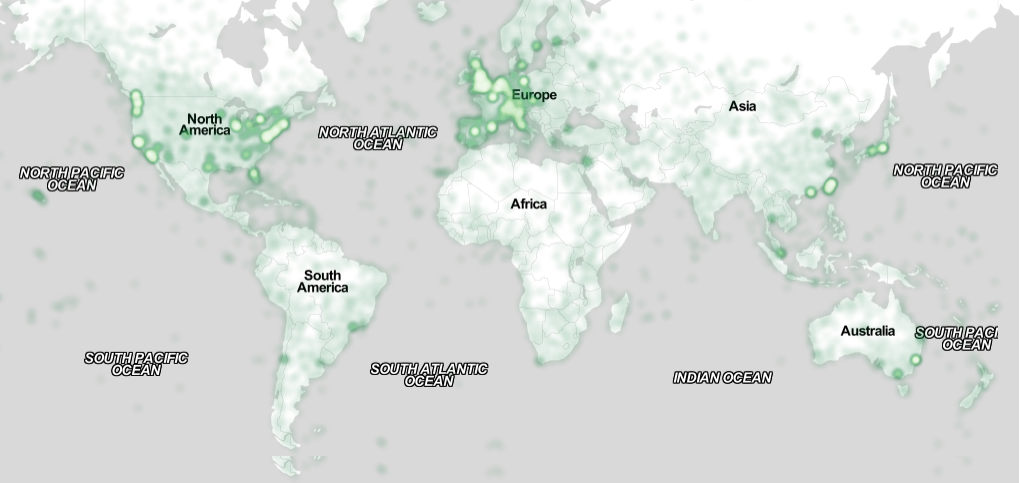
\includegraphics[width=300pt]{Images/map.png} % height 可以设置图片的高度, width 可以说设置图片的宽度
	\caption{样式1}\label{样式1} % label 用来在文中索引
	\vspace{-6mm} % 调整图片与下文的垂直距离
\end{figure}

下文······
% 图示例----------------------------------------------------------------------------------------

% 公式示例---------------------------------------------------------------------------------------
\section{\textcolor{blue}{\underline{\underline{公式-示例}}}}

\textcolor{blue}{公式标注应于该公式所在行的最右侧。对于较长的公式只可在符号处(+、-、*、/、$\leqslant$ $\geqslant$ 等)转行。在文中引用公式时,在标号前加“式”,如式(2-1)。}

% 公式上下不要空行,置于同一个段落下即可,否则上下距离会出现高度不一致的问题

\begin{equation}
	LRI=1\ ∕\ \sqrt{ 1 + {\left(\frac{{\mu}_{R}}{{\mu}_{s}}\right)^{2}}{\left(\frac{{\delta}_{R}}{{\delta}_{s}}\right)^{2}} }
\end{equation}
% 公式示例---------------------------------------------------------------------------------------

% 表示例----------------------------------------------------------------------------------------
\section{\textcolor{blue}{\underline{\underline{表-示例}}}}

\textcolor{blue}{{自动生成LaTeX表工具: \url{https://www.tablesgenerator.com/}}}

\begin{table}[htbp]
	\linespread{1.5}
	\zihao{5}
	\songti
	\centering
	\caption{物流的概念和范围}\label{物流的概念和范围}
	\begin{tabular}{|l|l|}
		\hline
		\multicolumn{1}{|c|}{本 质} & \multicolumn{1}{c|}{过  程}  \\ \hline
		途径或方法                     & 规划、实施、控制                   \\ \hline
		目标                        & 效率、成本效益                    \\ \hline
		活动或作业                     & 流动与储存                      \\ \hline
		处理对象                      & 原材料、在制品、产成品、相关信息           \\ \hline
		范围                        & 从原点(供应商)到终点(最终顾客)          \\ \hline
		目的或目标                     & 适应顾客的需求(产品、功能、数量、质量、时间、价格) \\ \hline
	\end{tabular}
\end{table}

% \begin{table}[htbp]
	%   \linespread{1.5}
	%   \zihao{5}
	%   \songti
	%   \centering
	%   \caption{统计表}\label{统计表}
	%   \begin{tabular}{|l|l|l|l|l|}
		%   \hline
		%   产品  & 产量    & 销量    & 产值   & 比重    \\ \hline
		%   手机  & 11000 & 10000 & 500  & 50\%  \\ \hline
		%   电视机 & 5500  & 5000  & 220  & 22\%  \\ \hline
		%   计算机 & 1100  & 1000  & 280  & 28\%  \\ \hline
		%   合计  & 17600 & 16000 & 1000 & 100\% \\ \hline
		%   \end{tabular}
	% \end{table}

\begin{table}[htbp]
	\linespread{1.5}
	\zihao{5}
	\songti
	\centering
	\caption{统计表}\label{统计表}
	% Please add the following required packages to your document preamble:
	% \usepackage{multirow}
	\begin{tabular}{|l|l|l|l|l|}
		\hline
		年度                    & 产品  & 产量    & 销量    & 产值  \\ \hline
		\multirow{2}{*}{2004} & 手机  & 11000 & 10000 & 500 \\ \cline{2-5} 
		& 计算机 & 1100  & 1000  & 280 \\ \hline
		\multirow{2}{*}{2005} & 手机  & 16000 & 13000 & 550 \\ \cline{2-5} 
		& 计算机 & 2100  & 1500  & 320 \\ \hline
	\end{tabular}
\end{table}
% 表示例----------------------------------------------------------------------------------------

% 伪代码示例------------------------------------------------------------------------------------

\section{\textcolor{blue}{\underline{\underline{伪代码-示例}}}}

\textcolor{blue}{修改 algorithmic 之间的代码就可以实现论文伪代码,已经考虑了伪代码跨页问题}
\begin{breakablealgorithm}
	\caption{Calculate $y = x^n$}
	\begin{algorithmic}[1] %每行显示行号
		\Require $n \geq 0 \vee x \neq 0$ 
		\Ensure  $y = x^n$
		\State $y \gets 1$
		\If{$n < 0$}
		\State $ X \gets 1 / x$
		\State $N \gets -n$
		\Else
		\State $X \gets x$
		\State $N \gets n$
		\EndIf
		\While{ $N \neq 0$ }
		\If{ $N$ is even }
		\State $X \gets x \times x$
		\State $N \gets N / 2$
		\Else[$N$ is odd]
		\State $y \gets y \times X$
		\State $N \gets N - 1$
		\EndIf
		\EndWhile
	\end{algorithmic}
\end{breakablealgorithm}
% 伪代码示例------------------------------------------------------------------------------------

% 代码块示例------------------------------------------------------------------------------------
\section{\textcolor{blue}{\underline{\underline{代码块-示例}}}}
\textcolor{blue}{只写了 C++, Python, Java 三种语言的格式}

% C++ 代码引入 + 文件引入
\lstinputlisting[
style = C++,
caption = {test.cpp},
label = {test.cpp}
]{./papperCode/test.cpp}

% Java 代码引入 + 行内引入
\begin{lstlisting}[
	style = Java,
	caption = {test.jar},
	label = {test.jar}
	]
	public class HelloWorld {
		public static void main(String[] args){
			System.out.println("Hello World!");
		}
	}
\end{lstlisting}

% Python 代码引入 + 文件引入
\lstinputlisting[
style = Python,
caption = {test.py},
label = {test.py}
]{./papperCode/test.py}
% 代码块示例------------------------------------------------------------------------------------